\chapter{Design of DevOps Toolchain}
In the chapter, we will first present the case software project that will be built, tested, and deployed by our DevOps toolchain in the experiment. Then we introduce the design and implementation of our DevOps toolchain which acts as the basis of our experiments in CH5. Note that
for the experiment that answering RQ 2, we implement two different continuous delivery pipelines design with two sets of tools respectively, one with tradition non-integrated tool while another one with the serverless integrated DevOps tools from AWS. In conclusion, we introduce the design of both toolchains(server-based and serverless) and explain how we come to this implementation in this chapter. 
\section{Case Project}
The case project is an example software project which will be used to test our implementation and run the experiments. This means we will simulate the DevOps development process of the case project on our DevOps toolchain. Although the type of our case project has no effect on our DevOps toolchain on the architecture level, the build dependencies and the software configuration inside our toolchain could be affected by it. Thus is necessary for us to have an introduction to the case project.
\subsection{Programming Language and Framework Considerations}
Java is one of the most common languages used in commercial software development. According to the TIOBE index of programming language \cite{indexTIO42:online}, Java is the most popular or the second most popular programming language in the world since the mid-1990s. Besides commercial software development inside companies, Java programming language is widely used in open-source software development. The report \cite{TheState3:online} from GitHub shows that Java ranks third most popular programming language in 2019, and it ranks second before 2018. Furthermore, Java has good versatility, which means it can be used in the development of almost every kind of applications. For instance, Java could be used for developing web applications, desktop applications, besides Java is the main development language for Android applications.
\par
To the DevOps point of view, the Java programming language has a very complete ecosystem. This means there are tools for every phase of Java application development. These tools include build, code analysis, testing frameworks, artifact management, build automation \& dependency management et. These tools could be easily integrated and act the part of the DevOps toolchain.
\par
Therefore, due to the popularity, versatility and complete ecosystem of Java programming language, we select Java as the language of the case project.
\par
One of the major application of Java in web development. Currently, 7 out of 10 \cite{Programm17:online} most popular website is using Java as a web development language (server-side). In the field of web development, Spring framework is the most popular framework for Java and it's being used in many major internet companies including Google, Microsoft and Amazon \cite{SpringWh14:online}. 
\par
So, we choose Spring the framework to build our application. To develop our Spring application, we use Spring Boot\footnote{https://spring.io/projects/spring-boot}. Spring Boot is a project under Spring, which according to its documentation, is to allow the developer to create Spring application with the minimal effort \cite{SpringBo84:online}, by simplifying the configuration of Spring framework. 
\subsection{Project Description}
\begin{figure}[!h]
    \begin{verbatim}
        Method: GET
        Endpoint: /packages
        Success Response:
            Code: 200
            Content: 
            [
                {
                    name : (Package name)
                    description : (Package description)
                    dependencies : (Dependencies) 
               }
            ]
        Error Response:
            Code: 500
            Content: { msg: Server Error! }
        \end{verbatim}
        \label{fig:rest}
\caption{RESTful API Interface of Case Project}      
\end{figure}
The case project is a simple REST API (Figure \ref{fig:rest}) which returns the info of all installed software packages in the host machine in JSON format when the frontend sends an HTTP GET request to the backend.
\section{Design of Non-integrated DevOps Toolchain}
In section, we present our design of  DevOps toolchain which is non-integrated. Part of the components is still based on the virtual machine. Each section is the introduction to the design of each component. We also present the consideration when a select tool for this part of the toolchain in each section. Besides, in each section, we introduce how could serverless computing be used by this component in general and the benefits to the specific tool we select.
\subsection{Architecture}
\begin{figure}[!htbp]
    \centering
    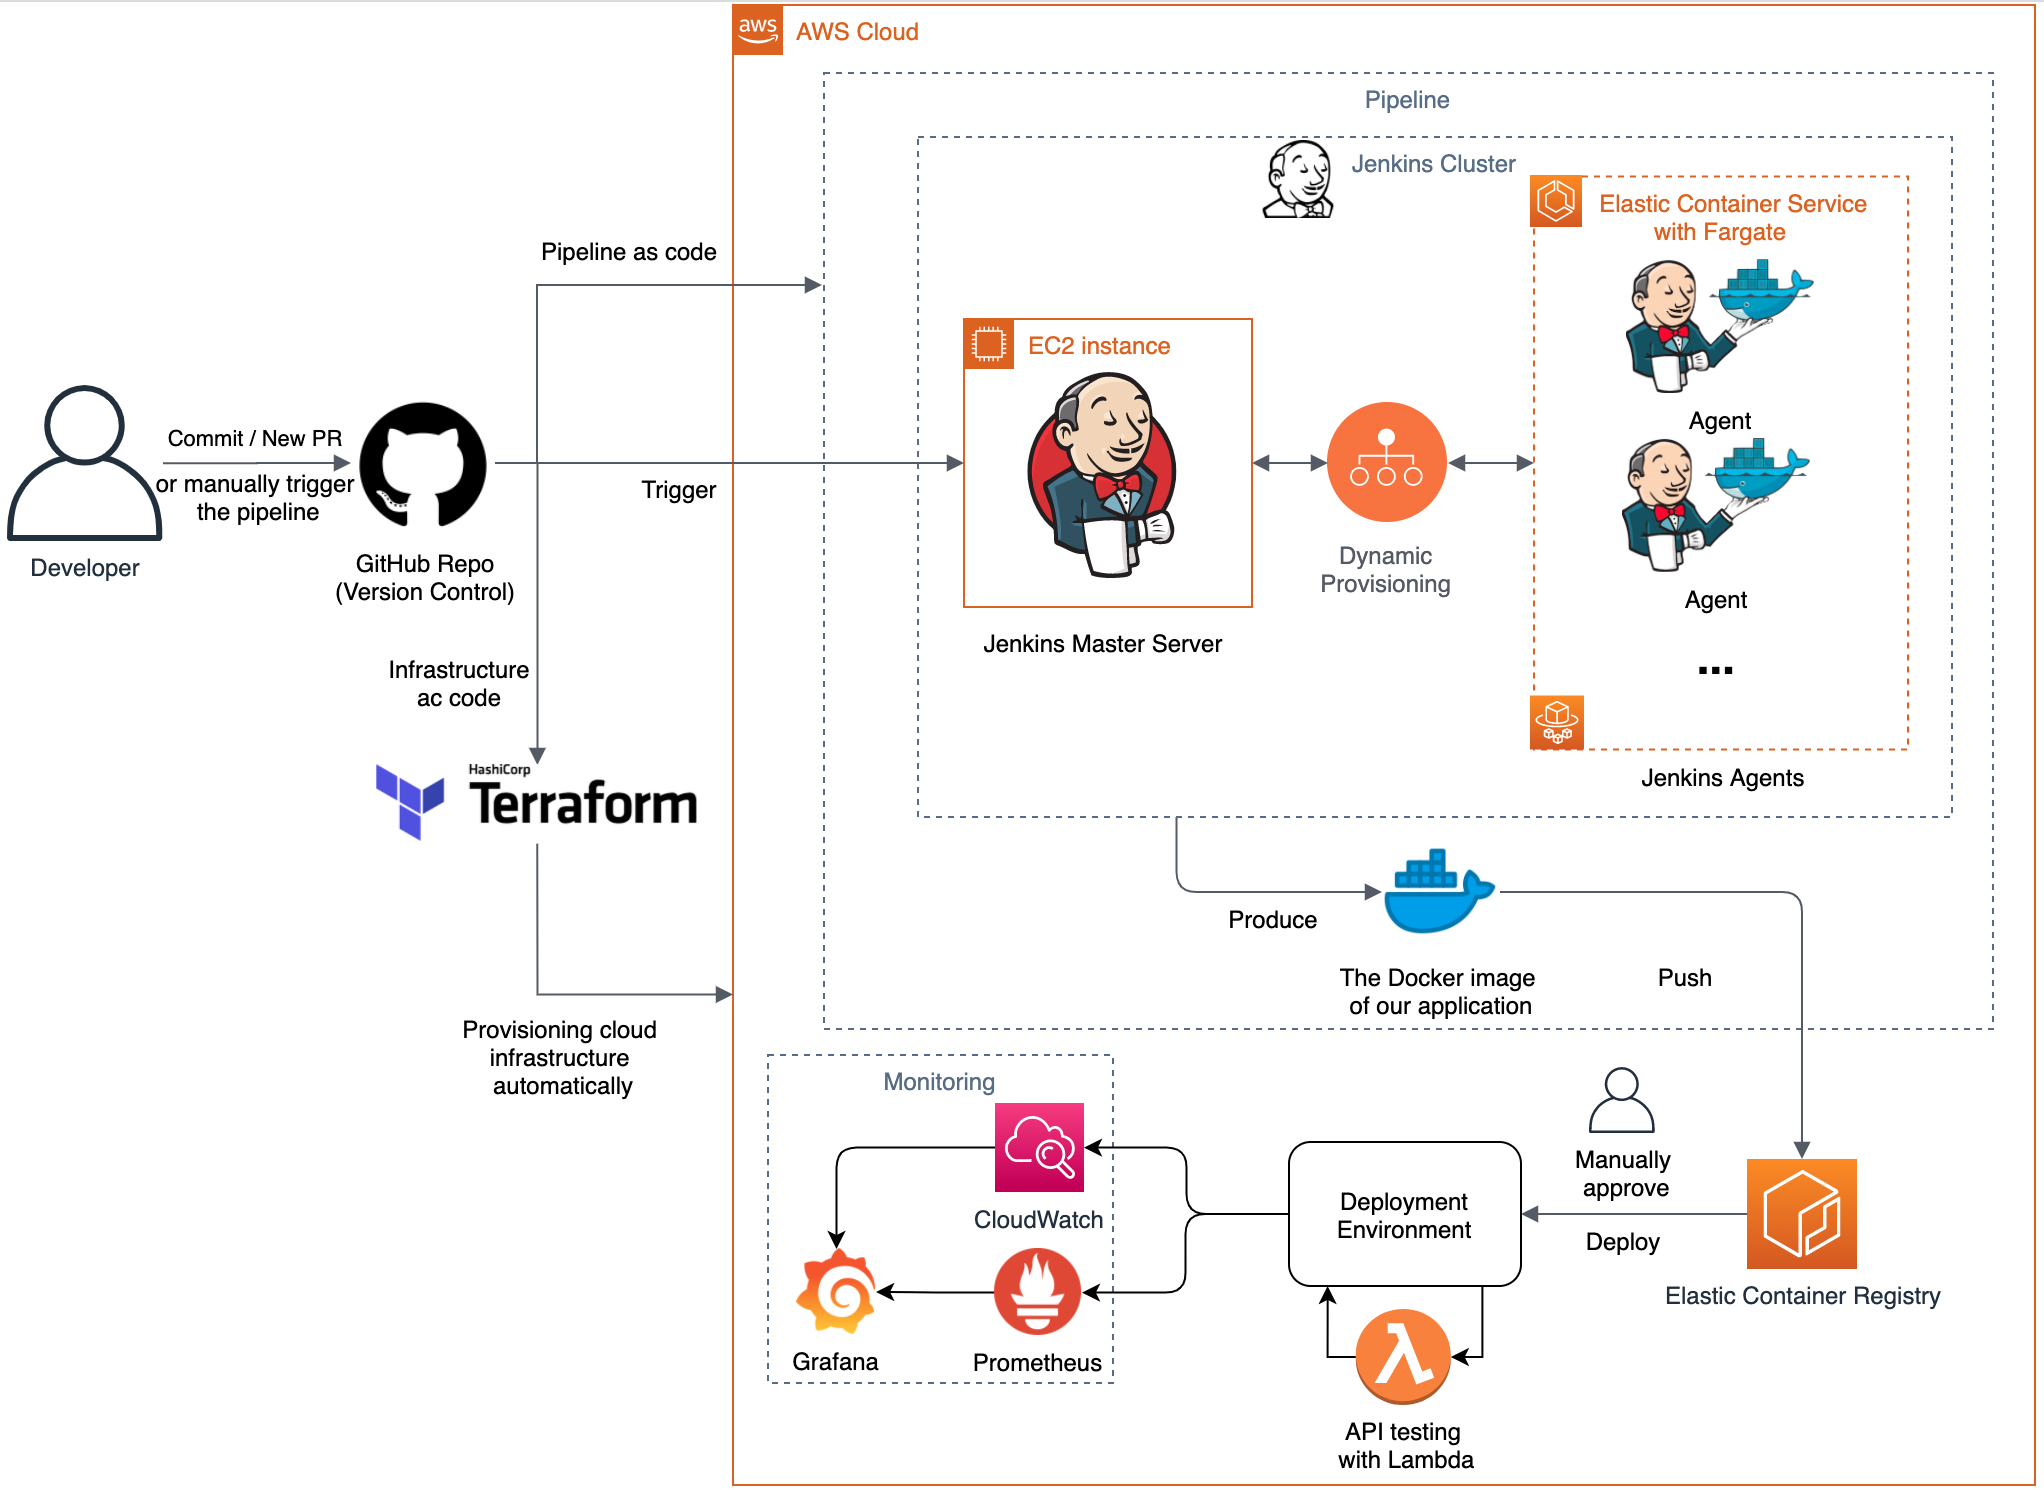
\includegraphics[width=0.99\textwidth]{pics/arch-med-jenkins.png}
    \caption{Architecture diagram of our DevOps toolchain}
    \label{fig:archjenkins}
\end{figure}
The toolchain implementation is based on the DevOps elements we presented in Chapter 2, and the DevOps practises from Eficode. Figure \ref{fig:archjenkins} shows the architecture of our DevOps toolchain. In here we only presenting architecture on a more general level. The detailed architecture of each component will be introduced in the following sections, in both text and graph.
\par
When the developer pushes a new commit to the repository in GitHub \footnote{https://github.com/}, Github will send an HTTP POST request that contains the necessary information to the Jenkins master node. Jenkins master which triggered by the HTTP request will create a new job for this project according to the information that the HTTP request contains. The job will first pull the latest code from the git repository, then runs the docker containers with required build environment and build the project. In the end, a docker image for running the project will be created and be pushed to the container registry of AWS. Depends on the git branch that the developer committed to, the project will be deployed to a different development environment.
\par
Figure \ref{fig:archjenkins} shows the architecture of our DevOps toolchain. We can see except version control, the whole environment is running in Amazon Web Services. Due to the limitation of space, the internal architecture of certain components is not shown in the graph, instead, we show them in the following sections.
\subsection{Version Control}
Version Control System (VCS) is the process that record the changes in files set over time \cite{GitAbout93:online}, and versioning the history of these files. VSC is suitable for track the development progress and manages the goal within a software development team \cite{loeliger2012version}. Among all software for version control, Git is the most popular one nowadays. The survey \cite{CompareR31:online} from Synopsys shows that in 2019, 71\% of the project today is using Git as it's versioning system while SVN that ranks in second only be used in 25\% of the projects. We use Git as the version control system since it is used by most of the software development teams nowadays. We use GitHub for hosting the case project. Github is the biggest preform in the world that hosting a version-controlled software project for free using Git. It provides interfaces with different DevOps related tools which makes it easy to be integrated into all kinds of DevOps toolchains.
\begin{figure}[h]
    \centering
    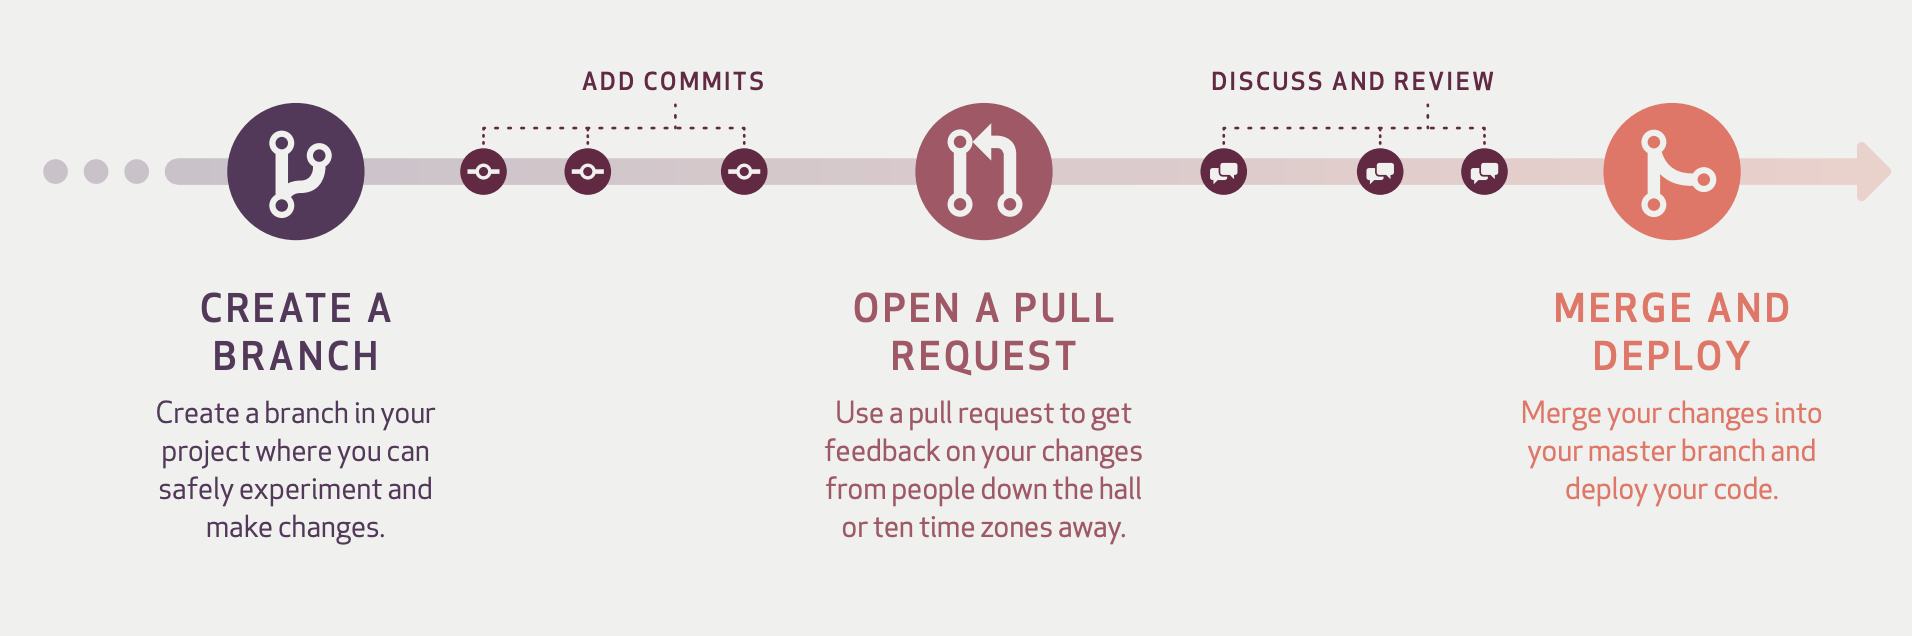
\includegraphics[width=0.99\textwidth]{pics/git.png}
    \caption{GitHub Workflow \cite{guides2013understanding}}
    \label{fig:git}
\end{figure}
\par
The Git flow \cite{driessen2010successful} proposed in 2010 is a successful workflow for working with Git. Git flow has already widely used and has been approved by the software industries. However, to better cope with the frequent release nature of DevOps, the Github workflow -- a simplified version of Git flow is proposed by GitHub.
Therefore GitHub workflow \cite{chacongithub} is being chosen as our workflow in the version control. The simplified version of this workflow is shown as in Figure \ref{fig:git}
\par
Several general principals followed by us when adapting GitHub flow, we refer the principals in \cite{chacongithub} to design our workflow.
\begin{itemize}
    \item Master branch is always deployable. This means when deploying the continuous delivery pipelines in our toolchain, only the master branch can be deployed. And there shouldn't have any code which is not good to be deployed in the master branch. 
    \item When working on the new feature, make a new branch for this feature. The name of this branch should be descriptive which reflect the content of this feature. Commit the code related to this feature this branch and push from this branch to the branch with the same name on the remote server (github.com).
    \item Open a pull request\footnote{https://help.github.com/en/GitHub/collaborating-with-issues-and-pull-requests/about-pull-requests} when the feature is ready to merge, or when you feel that you need help or comments from other team means on this feature. The code review is also done by others in the pull request.
    \item When the code is already be reviewed and is good to be merged, the developer should merge the code to the master.
    \item After the code of this feature is in the master, the code will and should be immediately deployed. There should not be any rollback in the master branch. If there are any issues within the newly merged code, a new commit or a new branch should be made to fix the issue rather than rollback on the master.
\end{itemize}
\par
Note that in our Git workflow, there are several time points that we need to run the continuous delivery pipeline within the toolchain. The continuous delivery pipeline will also vary with the time point within the version control workflow. We will introduce this in detail on \ref{our-ci}.
\subsection{Continuous Delivery Pipeline}
\label{our-ci}
\subsubsection{Tool Selection Considerations}
In this section, we describe about our consideration when select tools used in the continuous deliver pipeline.
\paragraph[]{Continuous Delivery Pipeline}
The most popular server-based tools for build continuous delivery pipeline are Jenkins\footnote{https://www.jenkins.io/}, Drone\footnote{https://drone.io/}, GoCD\footnote{https://www.gocd.org/} and Circle CI\footnote{https://circleci.com/}. A comparison between these tools is shown in Table \ref{tab:ci-tools}. As we can see from the table, Jenkins is the most popular option for CI/CD. Jenkins has wide application in the commercial use case, and the high popularity in the open-source community as well. Although compared with the other 3 newer tools, Jenkins is more focuses on the "Build" step within the continuous delivery pipeline. However, the open-source nature of Jenkins gives it a much wider selection of the plugin, which means Jenkins can be used for almost all steps in a continuous delivery pipeline. 
\begin{table}[h]
    \begin{tabular}{|l|l|l|l|l|}
    \hline
                        & Jenkins & Drone & Circle CI & GoCD \\ \hline
    Open Source         & Yes     & Yes   & No        & Yes  \\ \hline
    GitHub stars        & 15.7k   & 21.2k & -         & 5.7k \\ \hline
    Github contributors & 614     & 258   & -         & 116  \\ \hline
    Plugin extensions &
      Over 1500 \tablefootnote{https://plugins.jenkins.io/} &
      93 \tablefootnote{According to GitHub search result} &
      110 \tablefootnote{https://circleci.com/integrations/} &
      88 \tablefootnote{https://www.gocd.org/plugins/} \\ \hline
    \begin{tabular}[c]{@{}l@{}}Price of self-hosted \\ solution\end{tabular} &
      Free &
      Free &
      \$35 user/month &
      Free \\ \hline
    \begin{tabular}[c]{@{}l@{}}Number of companies\\use it in the tech stack\tablefootnote{based on data from StackShare}\end{tabular} &
      2634 &
      82 &
      1368 &
      42 \\ \hline
    \end{tabular}
    \caption{Comparison of continuous delivery tools}
    \label{tab:ci-tools}
    \end{table}
\par
Created by Kohsuke Kawaguchi in 2001, Jenkins is an open-source continuous integrating tool write with Java.  It is suitable for a team of all sizes and varies of languages and technologies \cite{smart2011jenkins}. Furthermore, Jenkins also attracts software teams with it's easy-to-use and high extendibility \cite{smart2011jenkins} with thousand of the plugin. More plugin keeps coming since Jenkins has an active open-source community. These plugins help Jenkins keep up with the fast-developing DevOps practices, and help Jenkins integrate with the newly emerging tools and cloud services. The extendibility makes Jenkins still the most popular tool for DevOps toolchain even it's an aged software created when the term "DevOps" just appeared.
\par
Our continuous delivery pipeline is built with Pipeline plugin\footnote{https://www.jenkins.io/doc/book/pipeline/} in Jenkins. 
Pipeline plugin allows us to define a continuous delivery pipeline as code in Jenkinsfile.
In the pipeline, a conceptually distinct subset of tasks within the continuous delivery pipeline \cite{Pipeline85:online} is defined as a "stage"\footnote{For example, "Build", Test", "Deploy" step in a continuous delivery pipeline.} and each task within a step is called "step". Each pipeline is binding with a "project". An execution runtime of a project/pipeline is called "build" and the machine (virtual machine, container, etc.) for running the build is called "agent".
\paragraph[]{Build \& Test Automation Tool}
For the build stage within Jenkins pipeline, we use Gradle\footnote{https://gradle.org/} as the build tool. 
Gradle is a powerful build tool initially designed for JVM based language, but now it also supports other programming languages, for example, C++ and Python. Like Jenkins, Gradle also has a dynamic ecosystem with thousands of plugin. This enables the possibility to use different kinds of tools such as unit testing and code analysis within a single pipeline of Gradle. Gradle also makes the dependency management easy, dependencies could be easily added to the project by editing the Gradle configure file of the project. Furthermore, Gradle supports configuration as code. This allows developers to define all of the build configurations of a software project in a single file.
\par
For unit testing within the build stage, we using JUnit \footnote{https://junit.org/junit5/} as the tool for testing. For code analysis, we use SonarQube\footnote{https://www.sonarqube.org/}. Both are one of the most common used tools in their specialized field in the Java ecosystem. And both tools have official Gradle plugin which allows us easily use them with Gradle. 
\paragraph[]{Deployment and Jenkins Agents}
We will widely use Docker \footnote{https://www.docker.com/} in our pipeline.  Docker is an open-source software which could pack, deliver and run the software as a container. A container is an isolated unit that includes the application and all its dependencies which allow application runs in the same way regardless of the host environment \cite{WhatisaC60:online}. A container is the running instance of a Docker image that defined by Dockerfile.
\par    
\label{docker}
There will be 2 main use cases of Docker in our toolchain. Firstly, we run the build stage within the container. To build the case application, the host machine needs to have JVM installed. However, we want to make our pipeline not only suitable for Java application but also easily be used to build an application in other programming languages. Docker solves this problem by provides good isolation from the host machine. Therefore we can configure the built environment (operating system version, dependencies) runs within Docker container  without actually install anything on the host machine by simply editing the Dockerfile.
\par
We also use Docker to Dockerize our application which creates a Docker image of our application.
Docker allows us to specify all system dependencies in a single file (Dockerfile), so there is no need to have any Java environment pre-installed in the deployment environment which runs our application. This is because all environment is already being packed in our Docker image. By doing this, firstly, we reduce the operational effort. Secondly, we improve compatibility since docker makes sure that the docker image could runs in the same behaviour no matter what host machine it runs on. Also, all major cloud computing providers support Docker. We could easily run the container from our Docker image on their VM and they're serverless computing services. This means our Dockerized application could easily be cloud-native and be deployed across a multi-cloud environment.
\subsubsection{Pipeline OverView}
\begin{figure}[h]
    \centering
    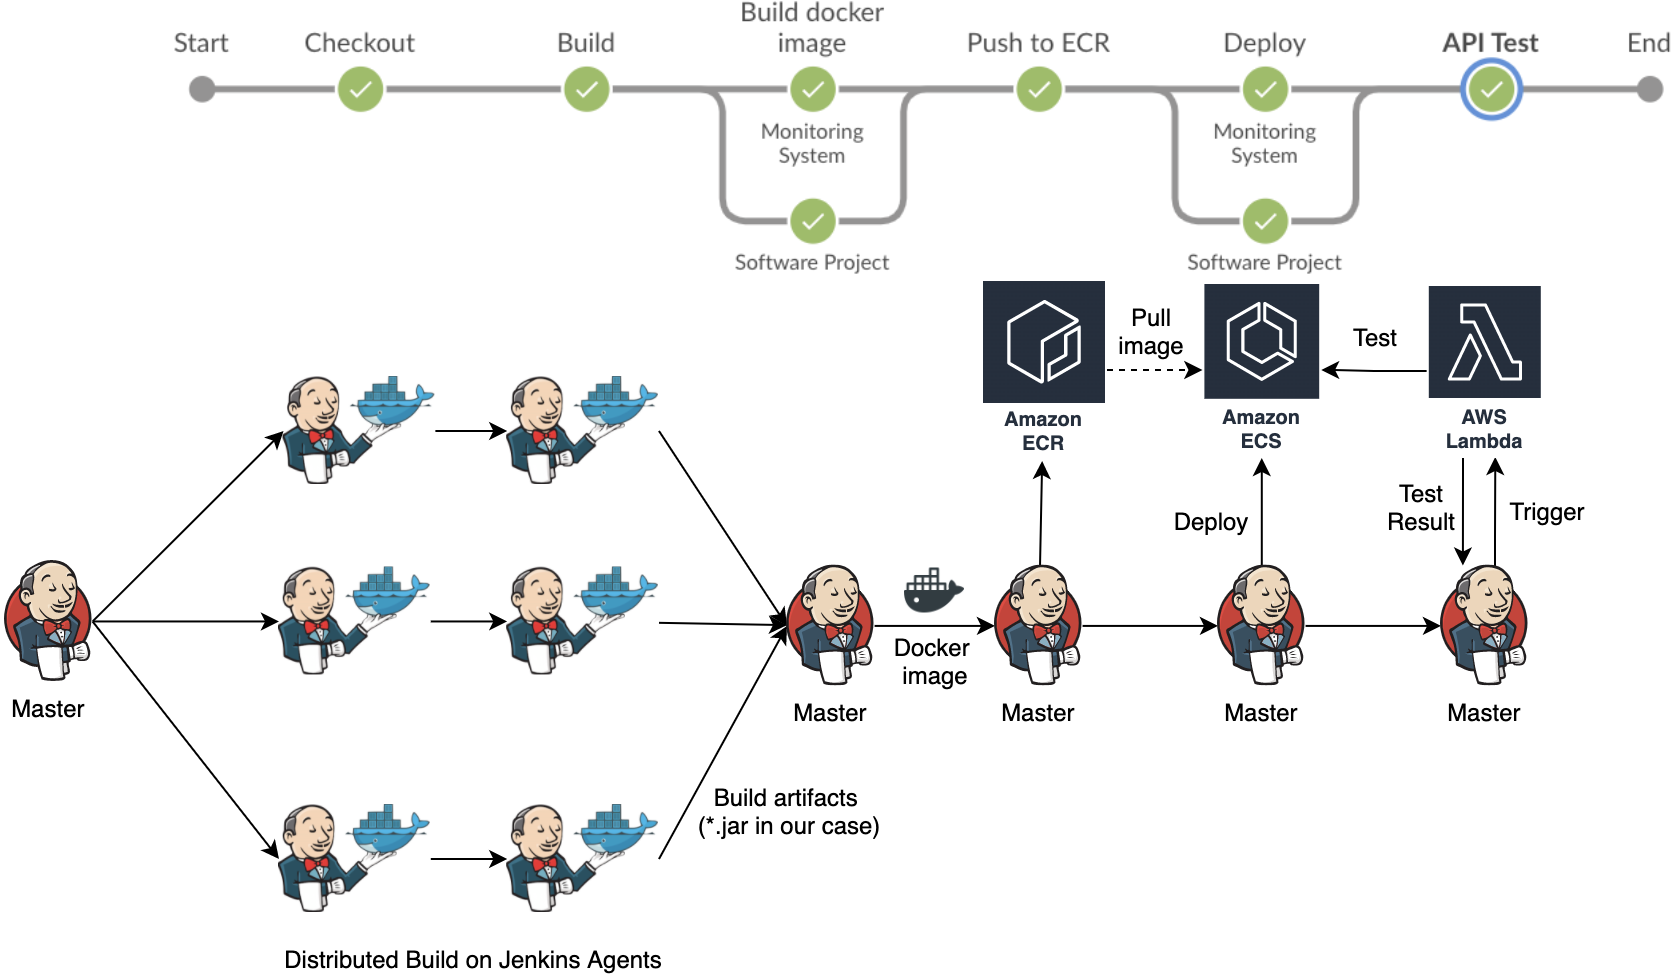
\includegraphics[width=0.95\textwidth]{pics/overview.png}
    \caption{The Stages and Distributed Build in Our Pipeline}
    \label{fig:overview}
\end{figure}
Figure \ref{fig:overview} shows the 5 stages in our pipeline that shown in the Jenkins dashboard. The bottom part of this Figure shows the task distribution between master node and agent nodes. 
As we can see from the figure, when the master node start a job, it will create Docker container in AWS Fargate as agent. The agent will pull codes from VCS, build the code, and then send the build artifacts back to master node. After this the container will be terminated. The master node will continue executes the rest steps.
\par
The considerations behind to our design is that, the first 2 steps takes most of time in our pipeline and according to Figure \ref{fig:pipeline} runs more frequently than other steps \footnote{The reason will be discussed in next section "Pipeline Workflow"}. The running time will be further extended when building larger project. These 2 stage will be the bottleneck of the pipeline if we have it on the master mode. So we need to offload these steps to Jenkins agents for better performance.
\par
The second reason is: as we mentioned in our introduction of Docker at \ref{docker}, the build environment inside Jenkins agents that runs in Docker container is easier to be changed. When the team want to build the same code for different OS (Which happens in C/C++ development) or want to have different build environment for different projects, they eliminates tasks such as configuration and installation different environment thanks to Docker. Instead, they can just modify the Dockerfile that defines the Docker image of the Jenkins agents.
\par
We also notice that the Deploy stage also takes long time. However, we don't have it in the distributed build because: first, it is on the end of a pipeline so it will not block te further steps, second, the pipeline runs ths stage less frequently than first 2 stages as shows in Figure \ref{fig:pipeline}, thus there will be less possibility that there are many jobs runs at "Deploy" stage in parallel.
\subsubsection{Pipeline Workflow}
Figure \ref{fig:pipeline} shows the workflow of a project that goes through our continuous delivery pipeline.
We can see when the pipeline is triggered by the event on the feature branch, it only runs through the first 2 stages. This is because according to the practices of continuous integration mentioned by us in \ref{CD} and by Martin Fowler in \cite{fowler2006continuous}, a developer should merge(the "integration" in continuous integration) his/her work couple times per day. Therefore the whole pipeline will run the code with this new feature at least several times a day. This already ensures the code could frequently be tested and deployed into the test environment. Thus, in the pipeline runs after the push to the feature branch the further steps could be skipped. 
\par
 The developer only commits to the feature branch. The pipeline runs first 2 stages after a developer pushes local commits to Git. It first pulls the newly pushed code, and then build. In the build stage, the code first is analysed, then we do unit testing to make sure the code could pass the test cases defined by the developer during development. In the end, the code will be built into Java ARchive file (.jar). The purpose of putting code analysis step first is that the code analysis will check syntax error and bugs. We want to make sure the code is runnable and no syntax error before put it into the build. So we can reduce the cost by reducing pipeline running time if there is error exists in the code. 
\par
If all the above steps are done and no error returns, the developer can open a pull request view the code change and ready to merge the code to the dev branch. Before the merge, the pull request needs to pass the code review by another developer. This is to make sure that the automated tests don't miss any bugs. After the code review passed, the reviewer or the developer him/herself merge the code to the dev branch.  
\par
After the code merged to the dev branch, the pipelines run again, this time it runs the whole pipeline. First, the pipeline executes the first two stages as in the feature branch. Now we have the Java ARchive file. The Java ARchive is an executable package of our Spring Boot application. Next step is to Dockerizing our application which generates the Docker image our application, and then we push the image to the Amazon Elastic Container Registry AWS (AWS ECR) for further use.
\par
\label{deploy}
The last step of the pipeline is deployment, the pipeline pull image in ECR that we pushed in the last stage, and then deploy it to the deployment environment. In our case, we using AWS Elastic Container Service (ECR) on AWS Fargate to host our application. As we mentioned in the CH3, it allow us to run our containerized application without having to manage servers. So it is easier for us to make an functionality complete DevOps toolchain implementation compared with server based deployment environment, for example AWS Elastic Kubernetes Service (EKS). 
During deployment we use Martin Fowler's blue and green deployment strategy \cite{fowler2010bluegreendeployment} which is natively supported by ECS. This means when a new deployment comes, the older version will continue serving until the newer version reach the stable status. This could significantly reduces the downtime in the deployment. 
\par
In the dev branch, we deploy the application to the staging environment. The deployment to staging environment should be automate, this is because the staging environment is only for testing, and only visible within the team. 
In the staging environment, we will conduct API smoke testing \cite{Smoketes27:online}. This is for test if our deployed API works and if it works as expected. If the deployed function passes the smoke test, this shows the deployment works as expected and ready for the deployment. The developer could now open an pull request, merge code to master branch. The pipeline will runs again, and deploy the application to the production environment which is visible to the costumers.
\begin{figure}[h]
    \centering
    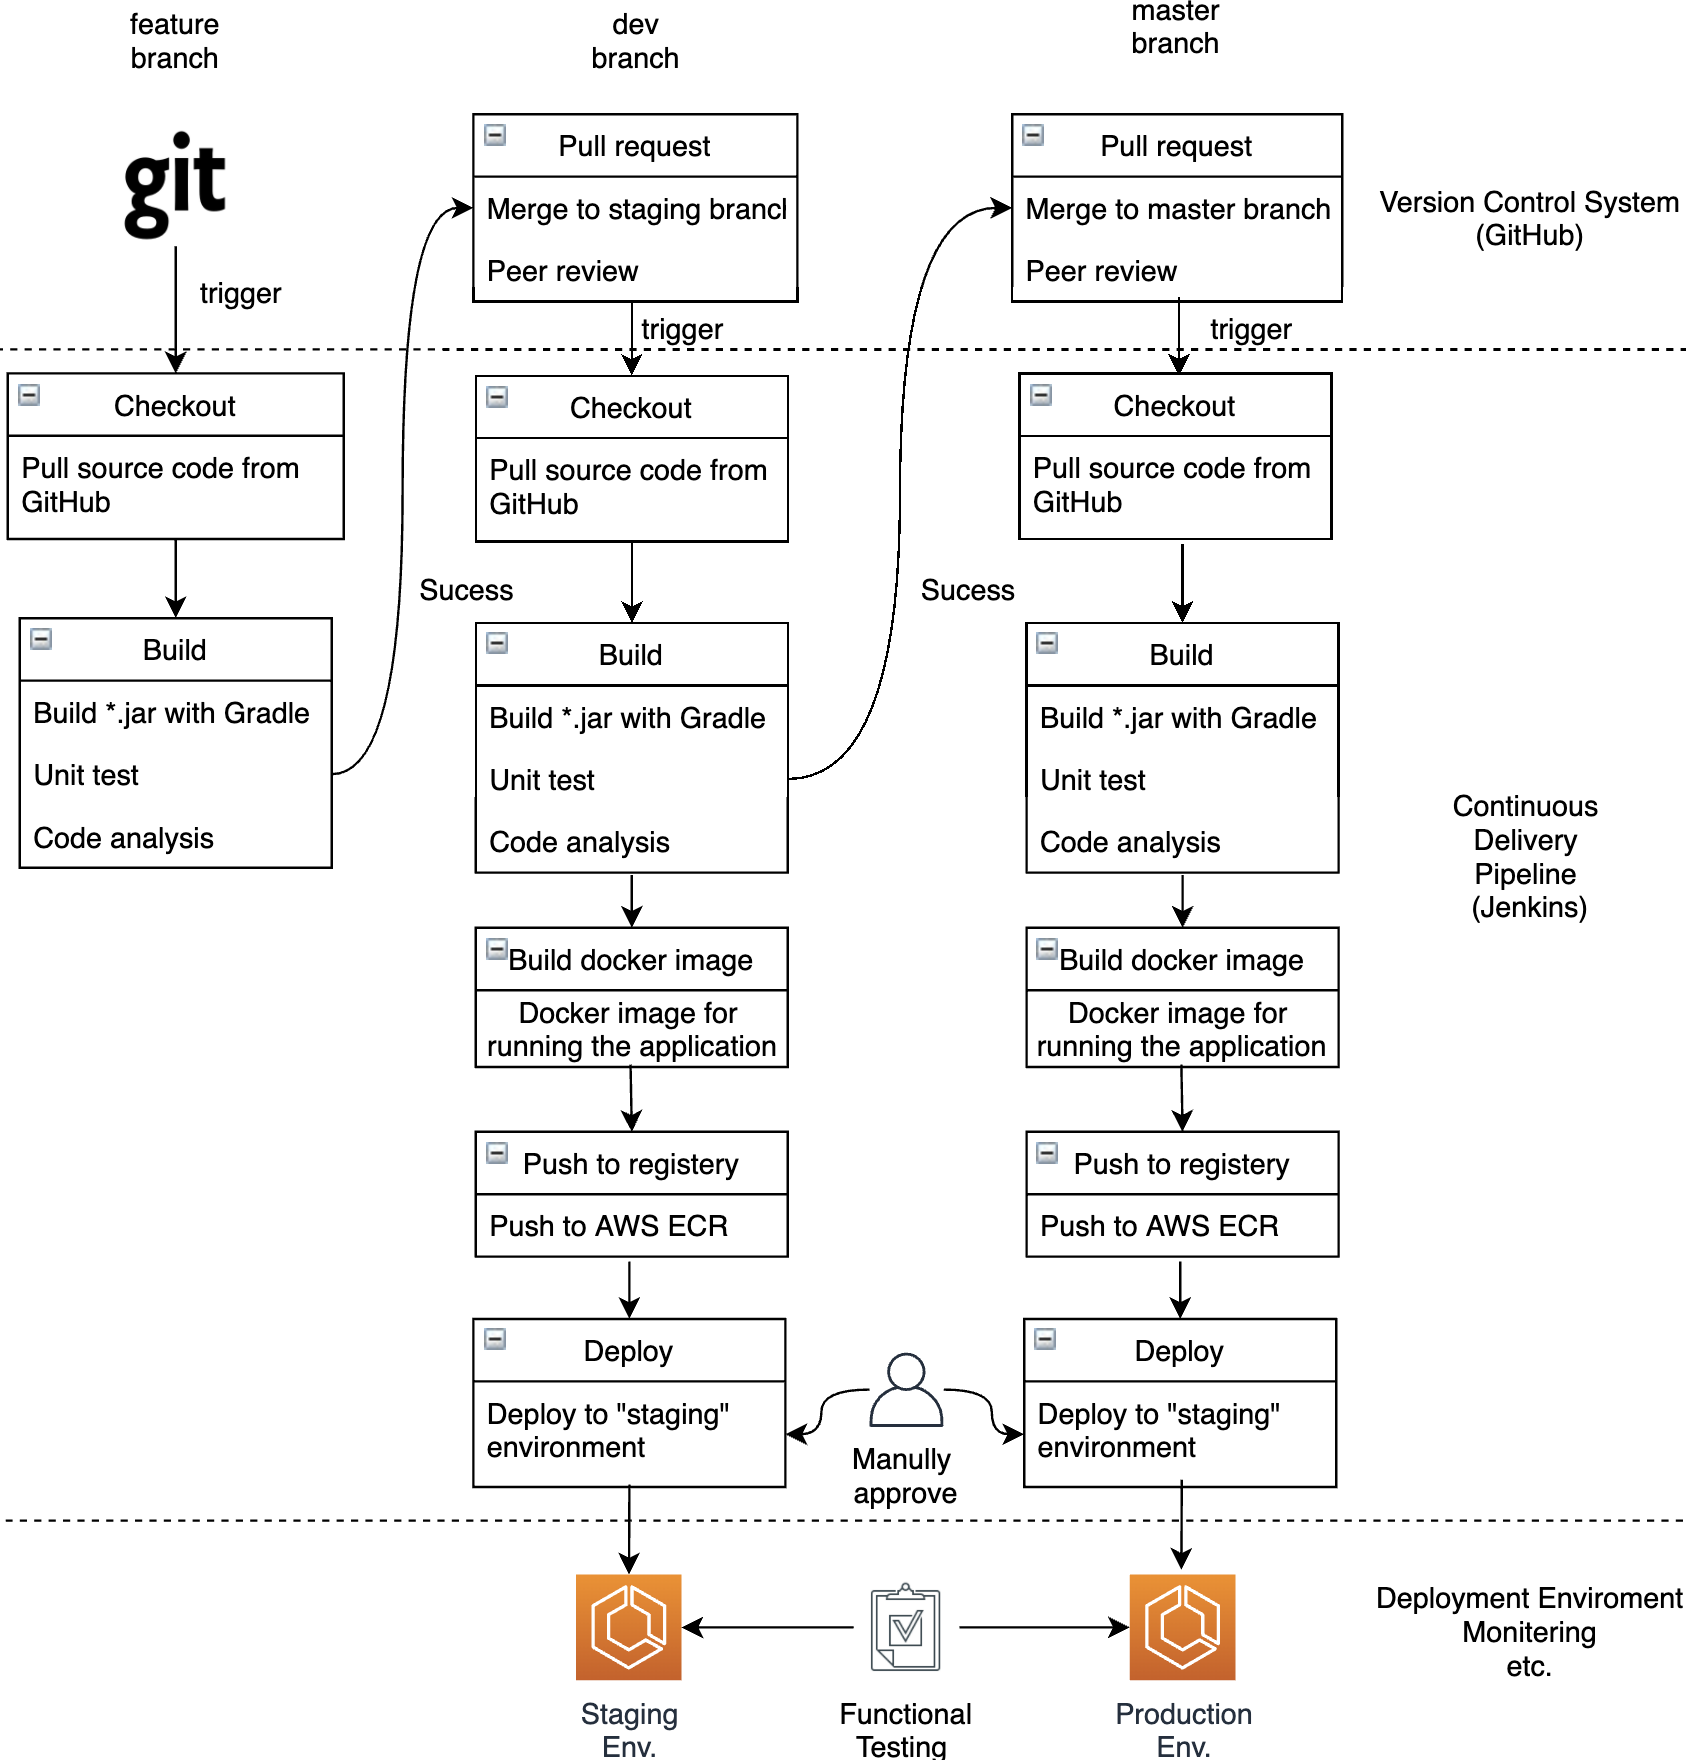
\includegraphics[width=0.99\textwidth]{pics/pipeline.png}
    \caption{The Workflow of Continuous Delivery Pipeline in Our DevOps Toolchain}
    \label{fig:pipeline}
\end{figure}

% \subsection{Smoke Testing}
% Testing is an implement component within the DevOps pipeline
% In this section, we further discuses about the smoke testing that we mentioned in the \ref{deploy}.
\subsection{Monitoring}
Monitoring is one of the important component in the DevOps toolchain. Different with testing which usually integrated with the continuous delivery pipeline, the monitoring is independent from the pipeline. Usually monitoring is not act as one step within the continuous delivery pipeline but as an independent component.
\par
In CH3 we introduced AWS cloudwatch as one of the serverless service in AWS. In our toolchain, we will use it as the primary tool for monitoring. Wih Cloudwatch, we not only can get the realtime log from our deployed container in the ECS, but also the quantitative data for example memory utilization and network i/o, the monitoring dashboard can be seem at figure \ref{fig:monitoring}
\begin{figure}[h]
    \centering
    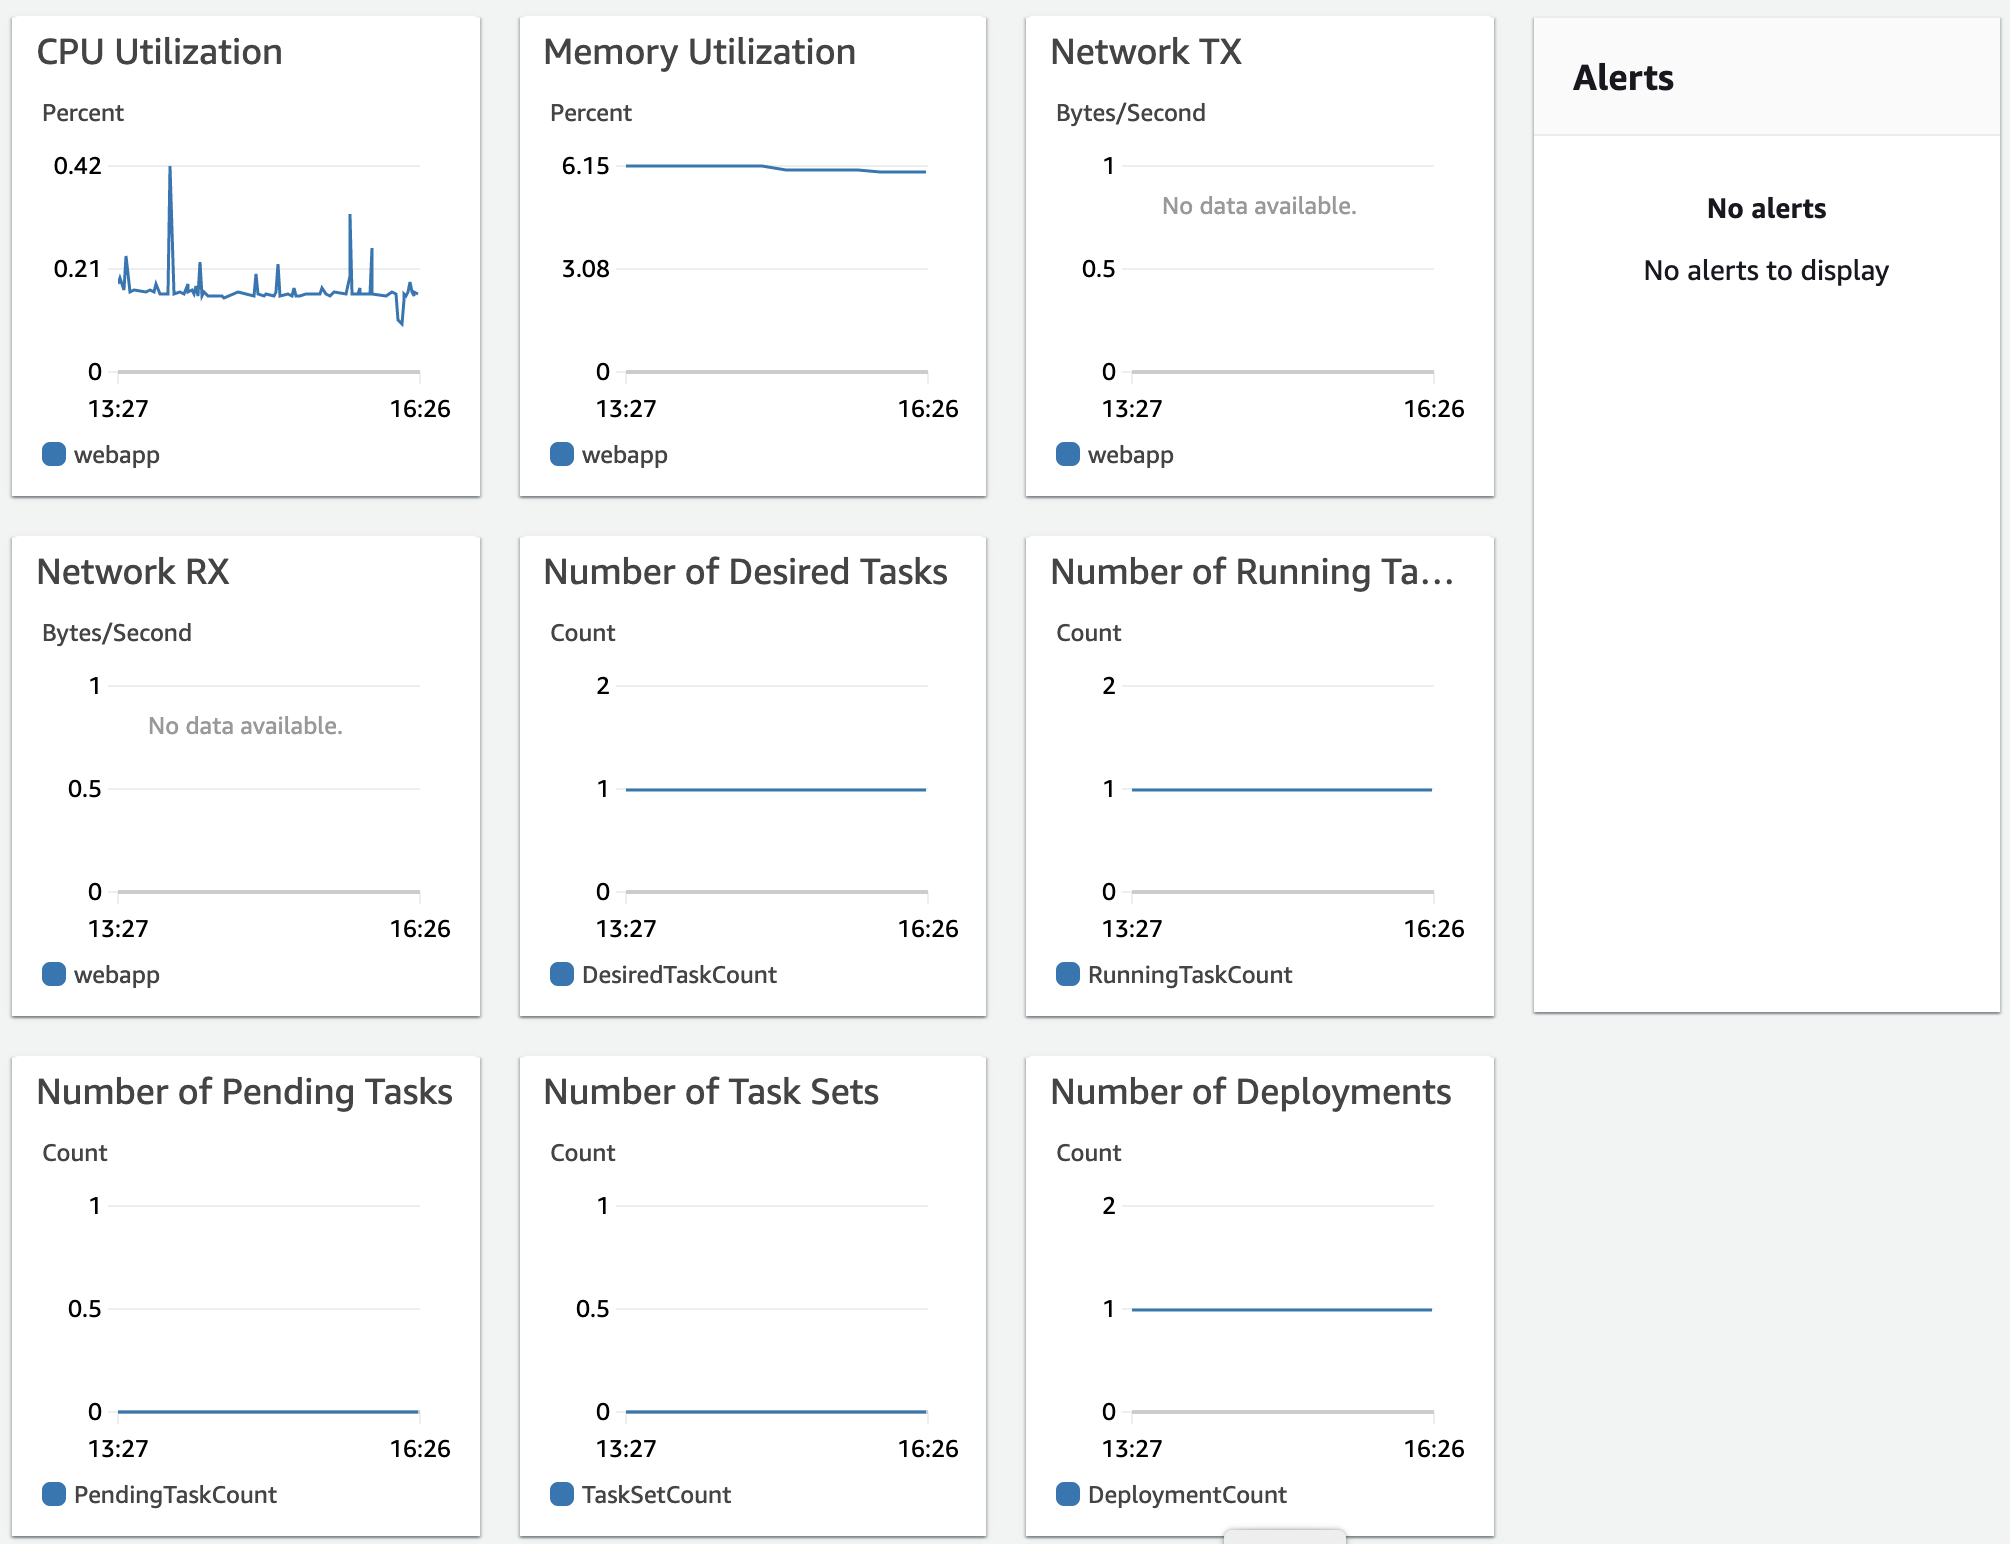
\includegraphics[width=0.70\textwidth]{pics/monitoring.png}
    \caption{Cloudwatch Monitoring Dashboard}
    \label{fig:monitoring}
\end{figure}
Another service we introduced in CH3 is AWS lambda. It is the most important serverless service in AWS. We also discussed how could it be used in our DevOps toolchain in which monitoring is one of the use cases. In our monitoring system, AWS lambda is used as an extension for cloud watch, and we use it for 2 cases.
\paragraph[]{Auto-Scaling the ECS Cluster with Alarm in Cloudwatch}

\paragraph[]{Custom Project-Specific Metrics}
\section{Design of Serverless DevOps Toolchain}
% \section{Cloud Services}
% \label{assumption}
% In this section, we will introduce several could service from CH3 that could be helpful to the DevOps toolchain. 
% //  Using services in AWS as an example, Introduces how cloud services could improve. describe services in one section
% \subsection{Managed Container Services for Distributed Builds} 

% // Describe how AWS Fargate could Help
% \subsection{Serverless computing}
% // Describe how AWS lambda could Help and why do we chose it
% \subsection{...}
